\chapter{Sistema de linealización, conversión punto flotante a punto fijo y normalización}

En la implementación del circuito completo se utilizan dos etapas, una para corriente del panel $i_{pv}$ y otra para la tensión del panel $V_{pv}$.

\begin{compactitem}

\item \nt{Corriente $i_{pv}$}: El bloque para la corriente requiere las etapa de linealización, conversión de la salida del linealizador de punto flotante a punto fijo, y un normalizador que da una salida de corriente entre el rango [-1,1].

\item \nt{Tensión $V_{pv}$}: La tension del panel se trabaja de manera lineal, de manera que solo se requiere de un normalizador que contenga la salida entre el intervalo [0,1]. 

\end{compactitem}

\begin{figure}[H]
  \centering
    \includegraphics[scale=0.04]{./Linealizador_normalizador.png}
    \rule{35em}{0.5pt}
  \caption[Sistema de linealización, conversión y normalización de corriente y tensión para un panel fotovoltaico]{Sistema de linealización, conversión y normalización de corriente y tensión para un panel fotovoltaico}
  \label{fig:Sist1}
\end{figure}


El sistema de la figura \ref{fig:Sist1} cuenta con 6 entradas y 4 salidas, estas se describen a continuación. 

Entradas:
\begin{compactitem}

\item \nt{CLK}: Reloj del sistema.
\item \nt{I}: Dato de corriente en formato IEEE 754
\item \nt{V}: Dato de tensión en formato IEEE 754
\item \nt{RST\_LN\_FF}: Reset para las unidades de corriente y tensión. 
\item \nt{Begin\_FSM\_I}: Inicia la máquina de estados del linealizador de corriente. 
\item \nt{Begin\_FSM\_V}: Inicia la máquina de estados de el convertidor punto flotante-punto fijo para la tensión. 

\end{compactitem}
Salidas:

\begin{compactitem}

\item \nt{ACK\_I}: Esta bandera indica que el resultado de las operaciones para la corriente se encuentra listo.  
\item \nt{ACK\_V}: Esta bandera indica que el resultado de las operaciones para la tensión se encuentra listo.  
\item \nt{RESULT\_I}: Resultado de corriente lineal y normalizado en formato punto fijo. 
\item \nt{RESULT\_V}: Resultado de de tensión normalizado en formato punto fijo.

\end{compactitem}

\begin{figure}[H]
  \centering
    \includegraphics[scale=0.05]{./Linealizador_normalizador2.png}
    \rule{35em}{0.5pt}
  \caption[Sistema de linealización-conversión-normalización de corriente y sistema de conversión- normalización de tensión para un panel fotovoltaico]{Sistema de linealización-conversión-normalización de corriente y sistema de conversión- normalización de tensión para un panel fotovoltaico}
  \label{fig:Sist2}
\end{figure}

La figura \ref{fig:Sist2} muestra la distribución de bloques funcionales para la corriente y tensión que proviene del panel fotovoltaico, todos los bloques se encuentran sincronizados con un mismo reloj $ \left(CLK\right)$ para la sección de corriente se realiza primeramente la linealización, iniciando con las señales RST\_LN\_FF y Begin\_FSM\_I y el dato de entrada I (corriente $\ i_{pv}$), una vez ejecutada la operación se envía una señal indicando que el dato esta listo ACK\_LN, esta se conecta a la señal de entrada e inicio del convertidor-normalizador de corriente Begin\_FF, justamente un ciclo de reloj antes de que esta señal de control se envíe, el resultado de la linealización $ \left(RESULT\right)$ esta listo, este está conectado a la entrada F del convertidor-normalizador, la ejecución de este se comprueba con la señal ACK\_I en donde se indica que la conversión-normalización fue realizada y el resultado se encuentra en RESULT\_I (corriente lineal y normalizada en punto fijo  $\ y' $).    

El bloque de tensión funciona de manera similar al de corriente, iniciando con las señales RST\_LN\_FF y Begin\_FSM\_V y el dato de entrada V (tensión $\ V_{pv}$), una vez ejecutada la operación se envía una señal indicando que el dato esta listo ACK\_V, el resultado se despliega en RESULT\_V (tensión normalizada en punto fijo  $\ z' $).

\section{Circuito para realizar las pruebas en Nexys-4}

Para desarrollar las pruebas dentro de la FPGA, se requirió diseñar e implementar un circuito para insertar datos a la entrada del linealizador-normalizador, sean procesados y posteriormente enviados por medio de transmisión serial hacia un computador.  

\begin{figure}[H]
  \centering
    \includegraphics[scale=0.06]{./test.png}
    \rule{35em}{0.5pt}
  \caption[Circuito de prueba para enviar datos por medio de UART desde la nexys-4 hacia un computador]{Circuito de prueba para enviar datos por medio de UART desde la nexys-4 hacia un computador}
  \label{fig:test}
\end{figure}

El diagrama de la figura \ref{fig:test} muestra el diseño del circuito utilizado, en donde se tiene una sección para ingresar 1024 datos, estos son almacenados en una memoria ROM, esta se carga por medio de un archivo de texto que contiene los datos de entrada para el linealizador-normalizador, esta memoria posee un contador para direccionar los 1024 datos. La sección de transmisión posee una unidad UART, esta se utiliza para enviar los resultados de la unidad de linealización-normalización hacia el computador, estos resultados tienen un formato punto fijo de 32 bits, el uart envía únicamente paquetes de 8 bits, por lo que se requiere enviar 4 paquetes por cada resultado, esto se logra por medio de una configuración de un multiplexor 4x1 y un contador, las entradas del multiplexor contienen el resultado dividido en paquetes de 8 bits y el contador selecciona el multiplexor según sea el paquete que se desea enviar. Por ultimo se cuenta con un control para el circuito, este se encarga de llevar la sincronía de los datos, primeramente se realiza una carga en el contador de la memoria ROM, este carga la primera posición de la ROM, posteriormente se inicia el procesamiento por parte de la unidad de linealización-normalización con la señal $\ Begin\_op$, el control espera a que el resultado este listo por medio de la señal ACK, cuando la condición ACK=High, el sistema se encuentra listo para transmitir, el contador del multiplexor selecciona el primer paquete y lo envía, el siguiente paquete se puede transmitir hasta que el modulo UART envié la señal $\ TX\_DONE$, así sucesivamente hasta que se envíen los 4 paquetes, cuando la selección del multiplexor esta en 2b'11 (contador del multiplexor), la señal $\ max\_tick\_mux$ indica al control que debe realizar una cuenta para la dirección de la ROM. Este proceso se repite hasta que la cuenta de las direcciones de la ROM es 1023 y la señal $\ max\_tick\_add = 1 $.
La recepción de datos desde el computador se realizo por medio del un puerto USB y un script realizado en Matlab, este recibe los paquetes de un byte en hexadecimal y los concatena en paquetes de 4 bytes, para formar el dato en 32 bits, posteriormente se convierte a decimal.   

\section{Simulación del sistema de linealización, conversión punto flotante a punto fijo y normalización implementado en hardware}

Este circuito se implementó por medio de la unión de los bloques anteriormente diseñados, implementados y simulados. 

\begin{figure}[H]
  \centering
    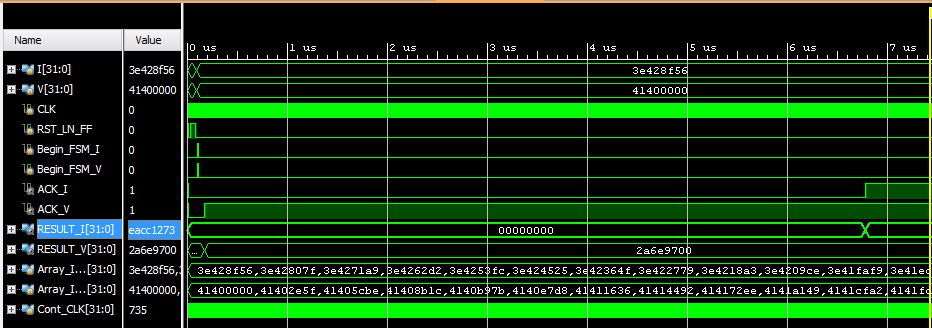
\includegraphics[scale=0.6]{./TEST_LINEALIZADOR_NORMALIZADOR.png}
    \rule{35em}{0.5pt}
  \caption[Simulación del sistema de linealización-conversión-normalización de corriente y sistema de conversión- normalización de tensión para un panel fotovoltaico]{Simulación del sistema de linealización-conversión-normalización de corriente y sistema de conversión- normalización de tensión para un panel fotovoltaico}
  \label{fig:Sim_Sist}
\end{figure}

La simulación básica "behavioral" efectuada por Vivado, verifica el funcionamiento adecuado del circuito a manera de software y de lógica sin embargo no es suficiente ya que se debe realizar la sintesis e implementación en verilog (Hardware), para esto se realizan las simulaciones post-syntesis y post-implementation, tanto del funcionamiento como de los retardos del sistema. La figura \ref{fig:Sim_Sist} muestra la simulación de tiempos posterior a la implementación.

\section{Resultados del sistema de linealización, conversión punto flotante a punto fijo y normalización implementado y verificado en hardware por medio de una FPGA nexys-4}

Las simulaciones para el circuito completo brindan una mejor información acerca del porcentaje de error total obtenido dentro de la conexión de las tres etapas  linealización, conversión y normalización. Se efectuaron las simulaciones de temporización y funcionalidad posterior a la síntesis, obteniendo resultados experimentales para realizar comparación contra los teóricos esperados.      
 
En el capítulo 3 se demostró el funcionamiento del linealizador con 8,12 y 15 iteraciones para el rango de convergencia del algoritmo de CORDIC, en este capítulo se utiliza el mismo principio de verificación, sin embargo se debe contemplar el error del normalizador, por lo que se realizan pruebas y comparaciones similares utilizando como datos de entrada un barrido de 1000 valores ingresados en el modelo teórico del panel fotovoltaico, esto con el fin de observar un comportamiento similar al real, estos valores de corriente son pequeños debido a la diferencia de corrientes y perdidas en el panel fotovoltaico, por lo que los porcentajes de error serán menores, ya que el circuito posee una mejor aproximación en el extremo inferior del intervalo de convergencia del algoritmo CORDIC. La visualización de los resultados obtenidos se realiza de una mejor manera mediante gráficos que indican como se comporta el circuito ante datos de entrada, salida, y porcentaje de error, apartir de los resultados de las simulaciones, se puede analizar la frecuencia de ejecución a la que se obtiene un resultado linealizado-normalizado, esta depende del numero de iteraciones que se utilice, por otro lado se deben sumar los ciclos de cada uno de los bloques funcionales que componen la ruta de ejecución de la corriente este circuito, se detallará de mejor manera en la siguiente sección.
Si tomamos el bloque para la tensión, este solo cuenta con la conversión-normalización y no depende del número de iteraciones por lo que se requieren de 8 ciclos de reloj por cada dato. 

\subsection{Sistema de linealización, conversión y normalización para la corriente $\ i_{pv}$ con 8 iteraciones implementado en una FPGA nexys-4} 
 
A partir de las simulaciones post-síntesis efectuadas por medio de la herramienta Vivado con una aproximación de 8 iteraciones, se puede observar que se requiere de 468 ciclos de reloj para completar la ejecución de un dato, este se compone de 460 ciclos de reloj para el linealizador y 8 ciclos de reloj para el convertidor-normalizador, donde la velocidad de ejecución es de 217kHz con un reloj de sistema de 100MHz.  

\begin{figure}[H]
  \centering
    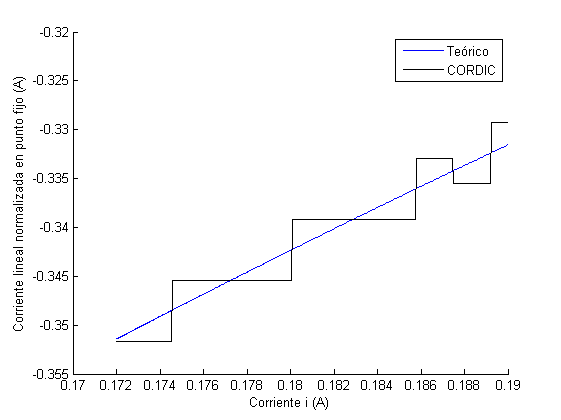
\includegraphics[scale=0.7]{./LINEALIZADOR_NORMALIZADOR_8iter.png}
    \rule{35em}{0.5pt}
  \caption[Comparación entre el valor teórico y el valor obtenido del circuito de linealización-conversión-normalización de corriente con 8 iteraciones en el algoritmo de CORDIC del linealizador]{Comparación entre el valor teórico y el valor obtenido del circuito de linealización-conversión-normalización de corriente con 8 iteraciones en el algoritmo de CORDIC del linealizador}
  \label{fig:LIN_NOR_8}
\end{figure}

\begin{figure}[H]
  \centering
    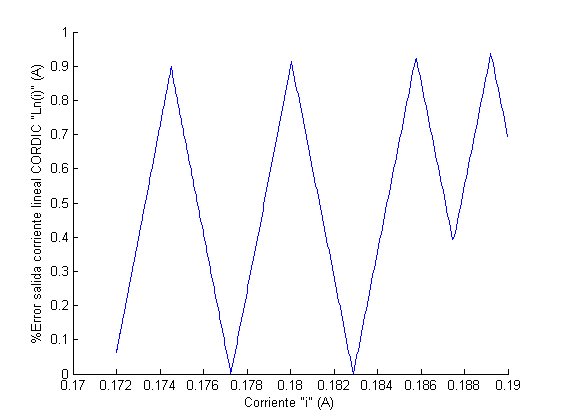
\includegraphics[scale=0.7]{./LINEALIZADOR_NORMALIZADOR_8iter_ERROR.png}
    \rule{35em}{0.5pt}
  \caption[Porcentaje de error entre el valor teórico y el valor obtenido del circuito de linealización-conversión-normalización de corriente con 8 iteraciones en el algoritmo de CORDIC del linealizador]{Porcentaje de error entre el valor teórico y el valor obtenido del circuito de linealización-conversión-normalización de corriente con 8 iteraciones en el algoritmo de CORDIC del linealizador}
  \label{fig:LIN_NOR_8_E}
\end{figure}

En la figura \ref{fig:LIN_NOR_8} se puede observar la comparación entre los datos obtenidos del circuito implementado en una FPGA nexys-4 contra los datos teóricos al realizar la misma función del circuito, debido a que son solo 8 iteraciones el circuito posee un resultados aceptables pero poco exactos, el gráfico muestra que el algoritmo trata de mantenerse cerca de los valores reales, sin embargo posee un comportamiento escalonado, en donde para cierta cantidad de valores de entrada posee un mismo valor de salida constante cercano al valor real. La figura \ref{fig:LIN_NOR_8_E} muestra el porcentaje de error asociado a cada valor de entrada linealizado y normalizado en formato punto fijo, donde el porcentaje de error máximo es de 0,922\% y un porcentaje de error promedio de 0,455\% esto para valores de corriente derivados a partir del modelo teórico del panel fotovoltaico. 
  

\subsection{Sistema de linealización, conversión y normalización para la corriente $\ i_{pv}$ con 12 iteraciones implementado en una FPGA nexys-4} 

Según las simulaciones post-sintesis del circuito con una configuración del algoritmo de CORDIC con 12 iteraciones, se requiere de 668 ciclos de reloj para realizar el procesamiento completo de un dato de entrada, 660 ciclos de reloj son utilizados por el linealizador y 8 ciclos de reloj para el convertidor-normalizador, con una velocidad de ejecución de 151kHz, utilizando un reloj de sistema de 100MHz.   

\begin{figure}[H]
  \centering
    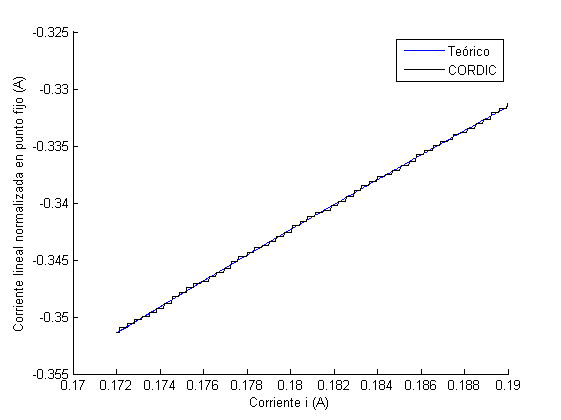
\includegraphics[scale=0.7]{./LINEALIZADOR_NORMALIZADOR_12iter.png}
    \rule{35em}{0.5pt}
  \caption[Comparación entre el valor teórico y el valor obtenido del circuito de linealización-conversión-normalización de corriente con 12 iteraciones en el algoritmo de CORDIC del linealizador]{Comparación entre el valor teórico y el valor obtenido del circuito de linealización-conversión-normalización de corriente con 12 iteraciones en el algoritmo de CORDIC del linealizador}
  \label{fig:LIN_NOR_12}
\end{figure}


\begin{figure}[H]
  \centering
    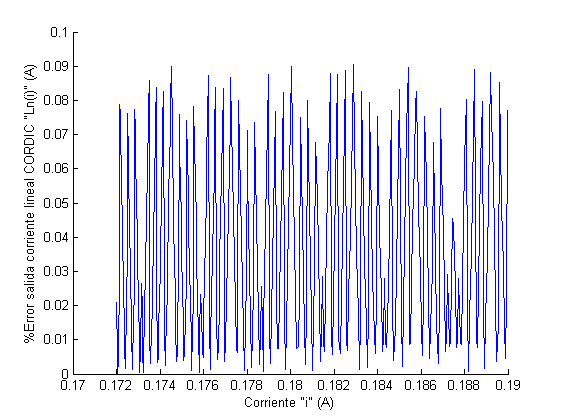
\includegraphics[scale=0.7]{./LINEALIZADOR_NORMALIZADOR_12iter_ERROR.png}
    \rule{35em}{0.5pt}
  \caption[Porcentaje de error entre el valor teórico y el valor obtenido del circuito de linealización-conversión-normalización de corriente con 12 iteraciones en el algoritmo de CORDIC del linealizador]{Porcentaje de error entre el valor teórico y el valor obtenido del circuito de linealización-conversión-normalización de corriente con 12 iteraciones en el algoritmo de CORDIC del linealizador}
  \label{fig:LIN_NOR_12_E}
\end{figure}

En la figura \ref{fig:LIN_NOR_12} se puede observar la comparación entre los datos obtenidos experimentalmente contra los datos teóricos al realizar la misma función del circuito, el uso de 12 iteraciones brinda una mejor exactitud contra 8 iteraciones, se puede observar que se presenta una mayor suavidad en la curva, sin embargo siempre se presenta un comportamiento escalonado pero con un valor mas cercano a la curva real. La figura \ref{fig:LIN_NOR_12_E} muestra el porcentaje de error asociado a cada valor de entrada linealizado con 12 iteraciones y normalizado en formato punto fijo, donde el porcentaje de error máximo es de 0,0897\% y un porcentaje de error promedio de 0,0345\% esto para valores de corriente derivados a partir del modelo teórico del panel fotovoltaico.


\subsection{Sistema de linealización, conversión y normalización para la corriente $\ i_{pv}$ con 15 iteraciones implementado en una FPGA nexys-4} 

En el sistema del panel es de suma importancia el tiempo de muestreo según sea la frecuencia del panel, esto implica velocidad de ejecución dentro del cálculo, se logró determinar que con 15 iteraciones se obtienen resultados con muy buena exactitud,sin embargo el tiempo de ejecución aumenta a 826 ciclos de reloj, tomando en cuenta que 818 ciclos son requeridos por el linealizador y 8 ciclos de reloj para la conversión de formato IEEE 754 a punto fijo y normalización, en donde la velocidad de ejecución es de 121kHz con un reloj de sistema de 100MHz.  


\begin{figure}[H]
  \centering
    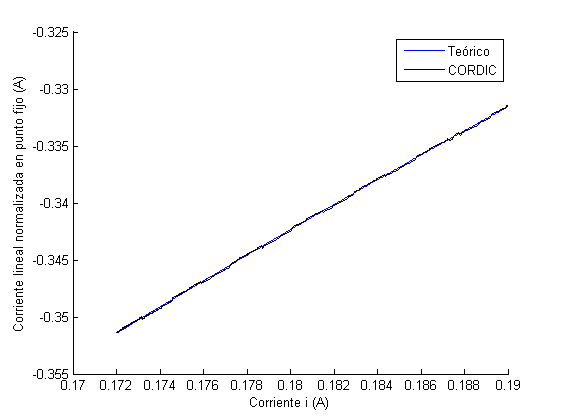
\includegraphics[scale=0.7]{./LINEALIZADOR_NORMALIZADOR_15iter.png}
    \rule{35em}{0.5pt}
  \caption[Comparación entre el valor teórico y el valor obtenido del circuito de linealización-conversión-normalización de corriente con 15 iteraciones en el algoritmo de CORDIC del linealizador]{Comparación entre el valor teórico y el valor obtenido del circuito de linealización-conversión-normalización de corriente con 15 iteraciones en el algoritmo de CORDIC del linealizador}
  \label{fig:LIN_NOR_15}
\end{figure}

\begin{figure}[H]
  \centering
    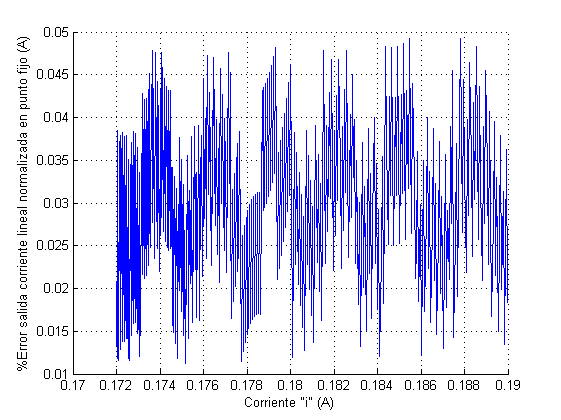
\includegraphics[scale=0.7]{./LINEALIZADOR_NORMALIZADOR_15iter_ERROR.png}
    \rule{35em}{0.5pt}
  \caption[Porcentaje de error entre el valor teórico y el valor obtenido del circuito de linealización-conversión-normalización de corriente con 15 iteraciones en el algoritmo de CORDIC del linealizador]{Porcentaje de error entre el valor teórico y el valor obtenido del circuito de linealización-conversión-normalización de corriente con 15 iteraciones en el algoritmo de CORDIC del linealizador}
  \label{fig:LIN_NOR_15_E}
\end{figure}

Con 15 iteraciones el valor experimental es muy similar al valor teórico, como se observa en la figura \ref{fig:LIN_NOR_15}, y se puede comprobar en la figura \ref{fig:LIN_NOR_15_E} donde se muestra que el porcentaje de error es muy cercano a cero, con un valor máximo de 0,0483\% y un error promedio de 0,0292\% esto para valores de corriente derivados a partir del modelo teórico del panel fotovoltaico.

El sistema de optimización se utilizará en un panel fotovoltaico que posee una frecuencia de 100kHz, es decir que el sistema de optimización debe realizar un cálculo completo velocidad mayor que el panel, aproximadamente el sistema de linealización y normalización toma un 40\% del total del tiempo de ejecución del sistema de optimización. Según lo anterior para realizar el cálculo en el tiempo indicado, el linealizador deberá utilizar 8 iteraciones.    


\section{Recursos utilizados}


\begin{table}[H]
\centering
\caption{Resumen del reporte post implementación del uso de dispositivos generado por la herramienta Vivado.}
\label{Table:Recursos}
\begin{tabular}{|c|c|c|c|c|c|}
\hline
Recurso & Utilizados  & Disponibles & Utilizados\%   \\ \hline

\begin{tabular}[c]{@{}c@{}} LUT
\end{tabular}  & 1017 &  63400   & 1.60      \\ \hline

\begin{tabular}[c]{@{}c@{}} FF
\end{tabular} & 912 & 126800   & 0.72         \\ \hline

\begin{tabular}[c]{@{}c@{}} DSP 
\end{tabular} & 4 & 240   & 1.67       \\ \hline

\begin{tabular}[c]{@{}l@{}} IO
\end{tabular} & 134 & 210   & 63.81     \\ \hline

\begin{tabular}[c]{@{}l@{}} BUFG
\end{tabular} & 1 & 32   & 3.12   \\ \hline

\end{tabular}
\end{table}

En la tabla \ref{Table:Recursos} se muestra el uso de recursos para la implementación el circuito completo en la Nexys4, el máximo recurso utilizado son los puertos I/O debido a que se requieren 32 bits en cada entrada I,V y 32 bits en cada salida RESULT\_I , RESULT\_V, sin embargo el uso de los demás recursos es sumamente bajo, el uso de los I/O se reducirá debido a que este circuito se deben acoplar a otro bloques del sistema de optimización.
  
\section{Reporte de tiempos}

Dentro del reporte de tiempos se analizan las peores rutas "ruta critica", para un buen diseño se requiere de slacks positivos, en el caso de "setup" un slack positvo indica que el dato llega a tiempo antes de ser utilizado, en el caso del "hold" indica que se mantiene por el tiempo adecuado antes de ser procesado por otro bloque, si ambos slacks son cero, el diseño esta en el limite y puede ser un poco arriesgado en sincronización. En la tabla \ref{Table:Tiempos} se muestran los valores obtenidos para los slacks del circuito del linealizador-normalizador.    

\begin{table}[H]
\centering
\caption{Resumen del reporte post implementación de tiempos del circuito completo, a partir de la herramienta Vivado.}
\label{Table:Tiempos}
\begin{tabular}{|c|c|c|}
\hline
Peor slack de todas las rutas & tiempo $ \left(ns\right) $      \\ \hline

\begin{tabular}[c]{@{}c@{}} Setup
\end{tabular}  & 0.459         \\ \hline

\begin{tabular}[c]{@{}c@{}} Hold
\end{tabular}  & 0.109          \\ \hline

\begin{tabular}[c]{@{}c@{}} Pulse width
\end{tabular}  & 4.5         \\ \hline


\end{tabular}
\end{table}

\section{Consumo de potencia}
Con la ayuda de las herramientas de análisis de potencia de Vivado, se pudo obtener los resultados que pertenecen al consumo de potencia, tanto estática como dinámica. En la tabla \ref{Table:Potencia1} se muestra el valor para cada consumo, y el total. 

\begin{table}[H]
\centering
\caption{Resumen del reporte post implementación de la potencia estática, dinámica y total, de la herramienta Vivado.}
\label{Table:Potencia1}
\begin{tabular}{|c|c|c|}
\hline
Potencia  & Consumo de potencia $ \left(mW\right) $      \\ \hline

\begin{tabular}[c]{@{}c@{}} Dinámica
\end{tabular}  & 11         \\ \hline

\begin{tabular}[c]{@{}c@{}} Estática
\end{tabular}  & 91          \\ \hline

\begin{tabular}[c]{@{}c@{}} Total
\end{tabular}  & 102         \\ \hline



\end{tabular}
\end{table}


Para los recursos utilizados se puede realizar un estudio de consumo de potencia dinámica, estos resultados se muestran en la tabla \ref{Table:Potencia2} donde el mayor consumo de potencia se presenta por parte del reloj del sistema y señales, las señales que poseen un valor de cero no se refieren a un consumo nulo, si no que es relativamente pequeño en comparación con las señales mas criticas.

\begin{table}[H]
\centering
\caption{Resumen del reporte generado por la herramienta Vivado que indica el consumo de potencia de diversos elementos. }
\label{Table:Potencia2}
\begin{tabular}{|c|c|c|c|c|c|c|}
\hline
On-chip $ \left(mW\right)$ & Consumo de potencia $ \left(mW\right) $      \\ \hline

\begin{tabular}[c]{@{}c@{}} Clocks
\end{tabular}  & 4          \\ \hline

\begin{tabular}[c]{@{}c@{}} Signals
\end{tabular}  & 4          \\ \hline

\begin{tabular}[c]{@{}c@{}} Logic
\end{tabular}  & 3          \\ \hline

\begin{tabular}[c]{@{}c@{}} DSP
\end{tabular}  & 0          \\ \hline

\begin{tabular}[c]{@{}c@{}} I/O
\end{tabular}  & 0          \\ \hline


\end{tabular}
\end{table}